\section{Architectures, Environment, and Applications}\label{sec:materials}
% follow bio papers: materials
% goal: 1.5 page
% table with comparison/differences
% incl non performance relevant info: name, type/domain, programming lang, etc., input type (dummy genome vs human genome, 3d sphere vs 2d stuff, etc); bytes-per-flop if in ref.?

%In this section we will mainly discuss the environment of our testing platforms and briefly introducing the benchmarks.
%In order to run our experiments, we need to setup our testing environment first.
Our research objective is to evaluate the impact of migrating from an architecture with (relatively) high amount of double-precision compute to an architecture with less. By high amount of double-precision compute we mean architectures whose Floating-Point Unit (FPU) has most of its silicon dedicated to 64-bit IEEE-754 floating-point operations, and by less double-precision compute we mean architectures that replace those same double-precision FPUs with lower -- potentially hybrid -- precision units.

%We are aware that several emerging application domains can aggressively exploit lower-precision arithmetic with little-to-no impact on solution quality, such as Deep-Learning~\cite{mixed_precision}. At the same time, we also know that many traditional applications demand double-precision arithmetic, and the applicability of hybrid precision in these is still an open research question. Finally, given that the trend in processor design seem to be re-allocating double-precision silicon to single- and half-precision units (e.g., Fujitsu's ARM64FX and NVIDIA's Volta-100), the question arises: How will the execution performance of these traditional application suffer (if at all?) when we migrate our HPC systems to host the new wave of processors?

To understand and explore the intersection of architectures with high-amount of double-precision and those with hybrid-precision, there is a need to find a processor whose architecture is unchanged with the sole exception of its floating-point unit to silicon distribution. Only one modern processor family allows for such an apples-to-apples comparison: the Xeon Phi family of processors.

\subsection{Hardware \& Software Environment}\label{ssec:hw}
%\cJD{fixed uncore freq!}
%\struc{small introduction sentence to this subsection and why it is relevant}
%\struc{introduce KNL KNM and BDW, HBM, outline reason for why we choose these}
%\struc{describe main differences between KNM and KNL which are important to our experiments, add or write about the VNNI changes}
%\struc{reference relevant work on how other centers run their phi and why they choose this}
%I have add one.
%\struc{describe the same OS, same SSD, same rack, same air cooling, same frequency setting, to minimize potential side-effects resulting in incorrect conclusions}
%As to find out if no more FP64 units are needed, we use KNL and KNM as our testing archetecture since they are the "most" equal architectures which just differ in FP64.
%We mainly do experiments on KNL and KNM architectures, also on Xeon Broadwell architecture as a validation. Table \ref{table:HW} shows the detailed information for each platform.
%\#INTRODUCTION FOR KNM KNL BDW HBM why choose
%KNL and KNM are released
%To make our experiments more convincing, we make sure that the severs we use for the experiments using the same OS, same SSD, same rack, same air cooling, same frequency setting, in order to minimize potential side-effects resulting in incorrect conclusions.
%Noted that, to make sure our tests are not disturbed by other users, we run all our tests exclusively.

\begin{table}[tbp]
    \caption{\label{table:HW} Detailed compute node hardware information; Differences between Knights Landing \& Mill highlighted in bold; Shown bandwidth (BW) measured with BabelStream (see Sec.\ref{ssec:bm}); Numbers for dual-socket reference system accumulated}
    \centering\scriptsize
    \newcommand{\tabincell}[2]{\begin{tabular}{@{}#1@{}}#2\end{tabular}}
    \begin{tabular}{|l|r|r|r|}
        \hline \hC
        \tH{Feature}                & \tH{KNL}                          & \tH{KNM}                          & \tH{Broadwell-EP} \\ \hline
        CPU Model                   & \textbf{7210F}                    & \textbf{7295}                     & 2x E5-2650v4              \\ \hline \rC
        \#\{Cores\} (HT)            & \textbf{64} (4x)                  & \textbf{72} (4x)                  & 24 (2x)                   \\ \hline
        Base Frequency              & \textbf{\unit[1.3]{GHz}}          & \textbf{\unit[1.5]{GHz}}          & \unit[2.2]{GHz}           \\ \hline \rC
        Max Turbo Freq.             & \textbf{\unit[1.5]{GHz}}          & \textbf{\unit[1.6]{GHz}}          & \unit[2.9]{GHz}           \\ \hline
        CPU Mode                    & Quadrant                          & Quadrant                          & \textit{N/A}              \\ \hline \rC
        TDP                         & \textbf{\unit[230]{W}}            & \textbf{\unit[320]{W}}            & \unit[210]{W}             \\ \hline
        DRAM Size                   & \unit[96]{GiB}                    & \unit[96]{GiB}                    & \unit[256]{GiB}           \\ \hline
        $\hookrightarrow$ Triad BW  & \textbf{\unit[71]{GB/s}}          & \textbf{\unit[88]{GB/s}}          & \unit[122]{GB/s}          \\ \hline \rC
        MCDRAM Size                 & \unit[16]{GiB}                    & \unit[16]{GiB}                    & \textit{N/A}              \\ \hline \rC
        %$\hookrightarrow$ Triad BW  & \unit[490]{GB/s} (flat;\cite{X})  & \unit[490]{GB/s}                  & \textit{N/A}         \\ \hline
        %\cJD{410GB/s seemed wrong, see \url{https://software.intel.com/en-us/articles/optimizing-memory-bandwidth-in-knights-landing-on-stream-triad}}
        $\hookrightarrow$ Triad BW  & \unit[439]{GB/s}                  & \unit[430]{GB/s}                  & \textit{N/A}              \\ \hline \rC
        MCDRAM Mode                 & Cache                             & Cache                             & \textit{N/A}              \\ \hline
        LLC Size                    & \textbf{\unit[32]{MiB}}           & \textbf{\unit[36]{MiB}}           & \unit[60]{MiB}            \\ \hline \rC
        Inst. Set Extension         & AVX-512                           & AVX-512                           & AVX2                      \\ \hline
        FP32 Peak Perf.             & \textbf{\unit[5,324]{Gflop/s}}    & \textbf{\unit[13,824]{Gflop/s}}   & \unit[1,382]{Gflop/s}     \\ \hline \rC
        FP64 Peak Perf.             & \textbf{\unit[2,662]{Gflop/s}}    & \textbf{\unit[1,728]{Gflop/s}}    & \unit[691]{Gflop/s}     \\ \hline
        %https://www.nas.nasa.gov/hecc/assets/pdf/training/Performance_Evaluation_Pleiades_Broadwell_Nodes.pdf
        %http://www.advancedclustering.com/wp-content/uploads/2017/02/xeon-e5v4.pdf
        %https://www.intel.com/content/dam/www/public/us/en/documents/white-papers/performance-xeon-e5-v3-advanced-vector-extensions-paper.pdf
        %\rowcolor[HTML]{C0C0C0}
        %\multicolumn{4}{|c|}{Hardware (other) } \\ \hline
        %SSD  &\multicolumn{3}{c|}{} \\ \hline
%        \rowcolor[HTML]{CCCCCC}
%        \multicolumn{4}{|c|}{Software} \\ \hline
%        OS          &\multicolumn{3}{c|}{Linux version 3.10.0-693.11.6.el7.x86\_64} \\ \hline
%        Compiler    &\multicolumn{3}{c|}{icc/ifort version 18.0.1 (gcc version 4.8.5 compatibility)}  \\ \hline
%        MPI         &\multicolumn{3}{c|}{Intel(R) MPI Library for Linux* OS, Version 2018 Update 1 Build 20171011} \\ \hline
\end{tabular}
        %\vspace{-1em}
\end{table}

%There are several differences between KNL and KNM many-core architectures. One of the main differences is single-/double-precision ratio. As is shown in Figure \ref{fig:knlvsknm}, KNM has half the DP flops/cyc while gets double SP flops/cyc compared with KNL. Which is an important reasion why we choose these two archetectures for our experiments.
\begin{comment}
\begin{figure}[tbp]
    \centering
    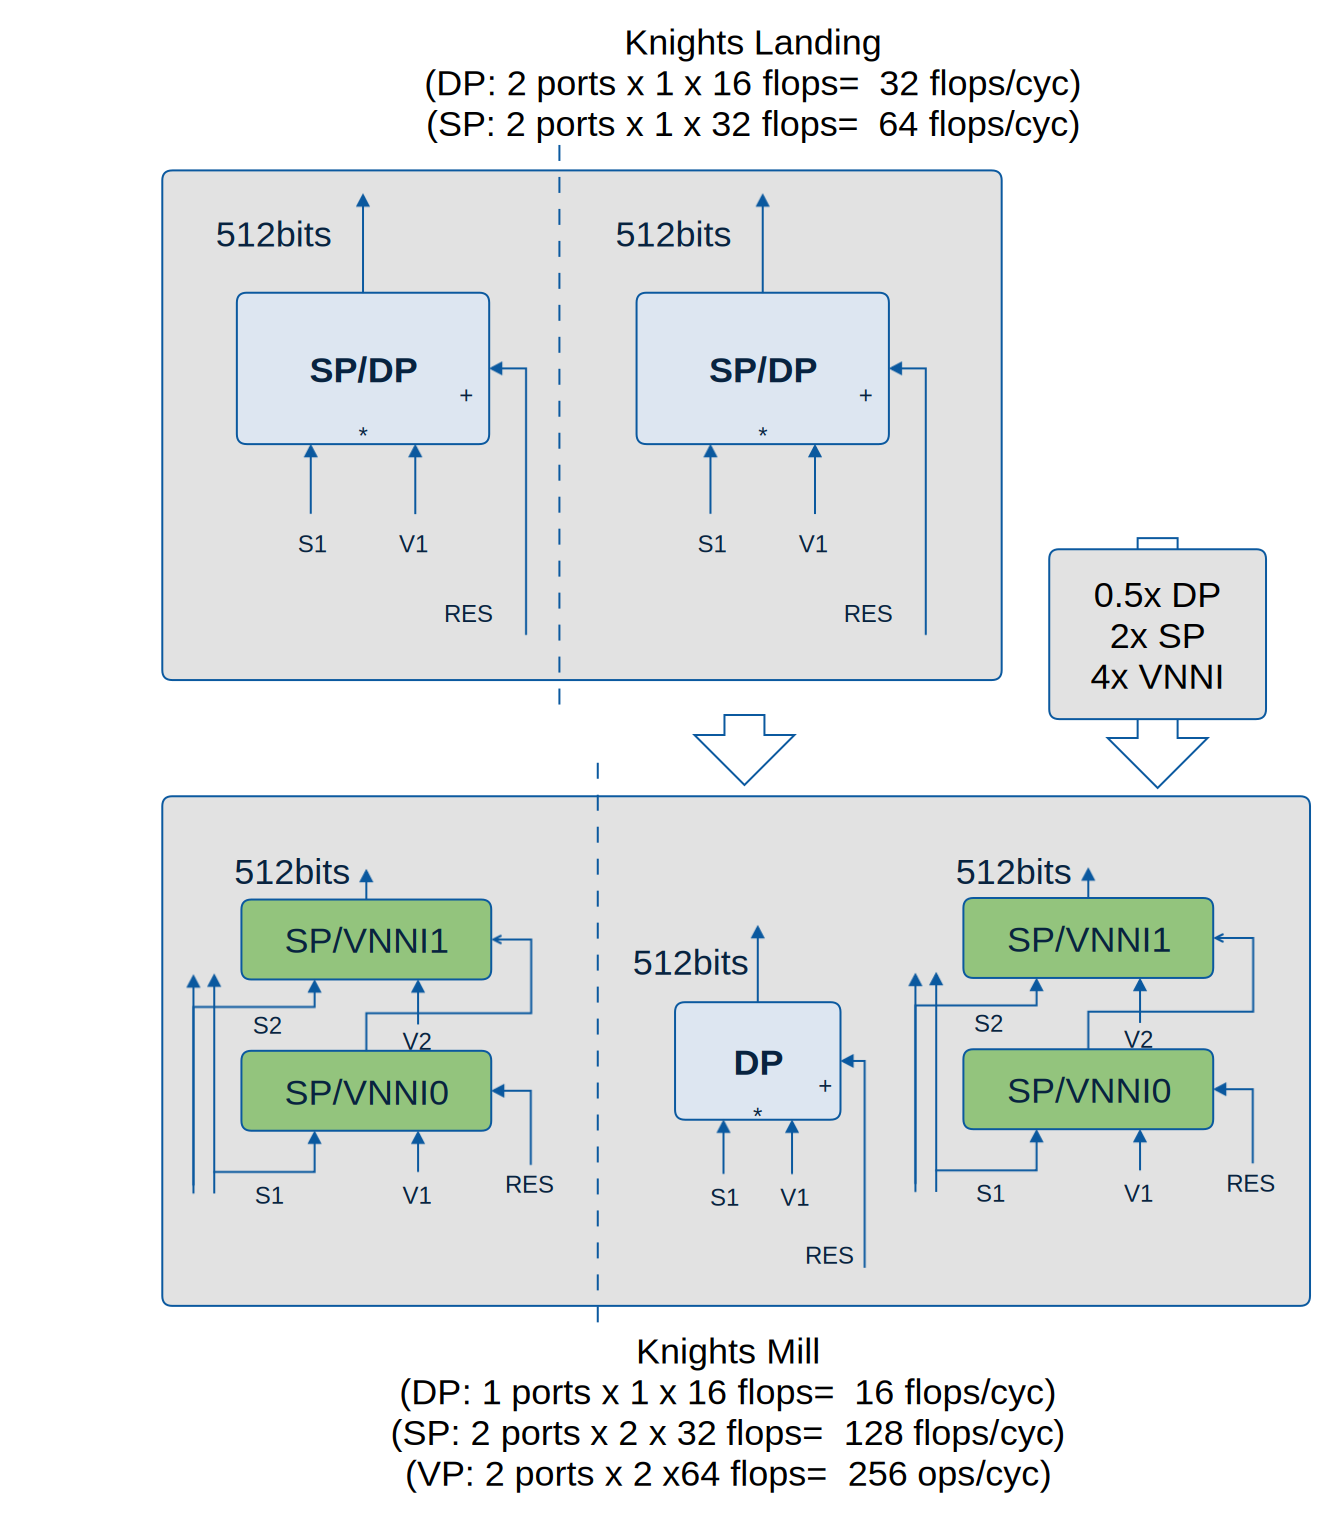
\includegraphics[width=.4\linewidth]{KNLvsKNM}
    \caption{\label{fig:knlvsknm}Comparison of KNL and KNM architecture\cJD{Is this figure necessary? Isn't Table 1 enough?}}
\end{figure}
\end{comment}

Intel's Knights Landing (KNL) and Knights Mill (KNM) are the latest incarnations of a long line of architectures in the Intel's accelerator family. Both processor consist of a large number of processors cores (64 and 72, respectively), interconnected in a mesh interconnection (prior to KNL: ring interconnection). Each core has a private L1 cache and a slice of the distributed L2 cache. Caches are kept coherent through the directory-based MESIF protocol.
Both processors come with two types of external memory: MCDRAM (or, Hybrid Memory Cube) and Double-Data Rate-synchronous (DDR4) memory. Unique to the Xeon Phi processors is that the MCDRAM memory can be configured to one of three modes of operation: it is either (1) directly addressable in the global memory address space (memory-mapped), called \texttt{flat} mode, or it (2) acts as last-level cache before the DDR, called \texttt{cache} mode. Finally, the third mode (hybrid mode~\cite{heinecke_high_2016}) is a combination of the properties from the first two modes.

There are several policies governing where data is homed. A common high-performance configuration~\cite{gawande_scaling_2017}, which is also the one we used in our study, is the quadrant mode. Quadrant mode means that the physical cores are divided into four logical parts, where each logical part is assigned two memory controllers; each logical group is treated as a unique Non-Uniform Memory-Access (NUMA) node, allowing the operating system to perform data-locality optimizations.
Table~\ref{table:HW} surveys and contrast the processors against each other, where the main differences are highlighted. The main architectural difference -- which is also the difference and its impact we seek to empirically quantify -- is the Floating-Point Unit (FPU). In KNL, this unit features two 512-bit wide vector units (AVX), together capable of executing 32 double-precision or 64 single-precision operations per cycle, totaling~\unit[2.6]{Tflop/s} of double- and~\unit[5.3]{Tflop/s} of single-precision performance, respectively, across all 64 processing cores. In KNM, however, the FPU is redesigned to replace one 512-bit vector unit with two Virtual Neural Network Instruction (VNNI) units. Those units, although specializing in hybrid-precision FMA, can execute single-precision vector instructions, but have no support for double-precision compute. Thus, in total, the KNM can execute up to~\unit[1.7]{Tflop/s} of double-precision or~\unit[13.8]{Tflop/s} of single-precision computations. In summary, the KNM has~2.59x more single-precision compute, while the KNL have~1.54x more double-precision compute.

While both the KNL and KNM are functionally and architectural similar, there are some note-worth differences. First, the operating frequency of the processors vary: the KNL operates at a frequency of~\unit[1.3]{GHz} (and up to~\unit[1.5]{GHz} in Turbo mode), while KNM operates at~\unit[1.5]{GHz} (\unit[1.6]{GHz} turbo). Hence, KNM executes~15\% more cycles per second over KNL. Furthermore, although the cores of KNM and KNL are similar (except the FPU), the number of cores are different: KNL has~64 cores while KNM has~72 cores. Both processors are manufactured in~\unit[14]{nm} technology. Finally, the amount of on-chip last-level cache between the two processors is different, where KNM has a~\unit[4]{MiB} advantage over KNL.

Additionally, for verification reasons, we include a modern dual-socket Xeon-based compute node in our evaluation. Despite being vastly different from the Xeon Phi systems, our Xeon Broadwell-EP (BDW) general-purpose processor is used to cross-check metrics, such as: execution time and performance (Xeon Phi should perform better), frequency-scaling experiments (BDW has more frequency domains), and performance counters (BDW exposes more performance counters).
Aside from those differences mentioned above (and highlighted in Table~\ref{table:HW}), the setup between the Xeon Phi nodes (and BDW node) is \textit{identical}, including the same operating system, software stack, and solid state disk. %(one Crucial mSSD SATA with \unit[480]{GiB} per node).

%\struc{add important notes on: linux kernel version and parameters, spector/meltdown patches, run levels, OS noise
%from NFS, other users, special settings to pre-installed OS/gnu/linux tools, ...; since we removed the info from the table}
For the operating system (OS) and software environment, we use equivalent setups across our three compute nodes.
The OS is a fresh installation of CentOS~7~(minimal) with Linux kernel version 3.10.0-862, which has the latest versions of
the Meltdown and Spectre patches enabled. During our experiments, we limit potential OS noise by disabling all
remote storage (Network File System in our case) and allowing only a single user on the system.
Most of our applications are compiled with Intel's Parallel Studio~XE (version 2018; update 3) compilers, and we
install the latest versions of Intel TensorFlow and Intel MKL-DNN for the deep learning proxy application, since
our assumption is that Intel's software stack allows for the highest utilization of their hardware.
Exceptions to this compiler selection are listed in the subsequent Section~\ref{sec:materials}.
We use Intel MPI from the Parallel Studio~XE suite to execute our measurements.

%Meanwhile, KNM has new instructions such as Quad Fused Multiply Add (QFMA),Variable precision instructions and Quad Virtual Neural Network Instruction (QVNNI). It is claimed by Intel that QFMA instructions enable 2x of the SP performance against KNL. Variable precision instructions help to get higher throughput in machine learning tasks. And QVNNI, the 16-bit INT operations are 4x faster than KNL's SP under the condition that Intel claims users can achieve “similar accuracy to single-precision.” with INT32 accumulated output.[see comment]
%[refer to slide https://indico.cern.ch/event/595059/contributions/2499304/attachments/1430242/2196659/Intel_and_ML_Talk_HansPabst.pdf]
%https://www.hpcwire.com/2017/06/22/knights-mill-gets-deep-learning-flops/
%One significant difference between Intel Xeon phi and Xeon is that Xeon phi have Multi-Channel DRAM (MCDRAM), which have a high bandwidth and relatively low capacity. There are several modes when using MCDRAM: cache mode, flat mode and hybrid mode.
%In cache mode, the MCDRAM will be performed as the last level cache. While in flat mode, MCDRAM will be used as memory. The hybrid mode is a mixture of the cache mode and flat mode.\cite{heinecke_high_2016}
%The mesh of Xeon phi can be operated in three different cluster modes: All2All mode, Quadrant mode and Sub-NUMA-Clustering(SNC4) mode.
%In All2All mode, no affinities are set. In Quadrant mode, the mesh will be divided into 4 logical parts and each memory controller will be mapped to one of four tag directories there belong to. For SNC4 mode, it is an extended version of the Quadrant mode, which exposes the four parts via NUMA domains to the OS.
%Nitin A. et al. in paper \cite{gawande_scaling_2017} discussed that which configuration should be chosen for a better performance. It is discussed that, cache mode + quadrant mode could be a better choice. Although AVX-512 instructions could benefit from flat mode, it need additional optimization to obtain the benefit.

\subsection{Benchmark Applications}\label{ssec:bm}

%\struc{small introduction sentence to this subsection and why it is relevant}

%\struc{introduce the ECP and postK mini-app projects, and why it is relevant for HPC and procurement}

%\struc{write short info about each application: what does it do, which science field it belongs to, what subproblem does the input data/parameter simulate, which category does it belong to (see riken study about code categories), byte2flop ratio if know from prev. publications}

Over the years, the HPC community developed many benchmarks representing real workloads or for testing the
capabilities of a system -- primarily for comparisons across architectures but also for system
procurement purposes.
The so-called Exascale Computing Project (ECP) proxy applications~\cite{noauthor_ecp_2018} and
RIKEN AICS' Fiber Miniapp Suite~\cite{riken_aics_fiber_2015}, which we will focus on for this study, are just
two examples representing modern HPC workloads.
Those benchmarks are designed to evaluate single-node and small-scale test installations,
and hence are adequate for our study.


\subsubsection{The ECP Proxy-Apps}\label{ssec:ecp}
The ECP suite (release~v1.0) consists of 12 proxy applications primarily written in C~(5x),
FORTRAN~(3x), C++~(3x), and Python~(1x), listed hereafter.

\paragraph{Algebraic multi-grid (AMG)} solver of the \textit{hypre} library is a parallel solver
for unstructured grids~\cite{park_high-performance_2015} arising from fluid dynamics problems.
We choose \textit{problem~1} for our tests, which applies a 27-point stencil on a 3-D linear system.
%https://github.com/LLNL/AMG/blob/master/docs/amg.README: AMG is also memory-access bound, doing only
%about 1-2 computations per memory access, so memory-access speeds will also have
%a large impact on performance.

\paragraph{CANDLE (CNDL)} is a deep learning benchmark suite to tackle various problems in cancer
research~\cite{wozniak_candle/supervisor:_2018}.
We select benchmark 1 of pilot 1 (\textit{P1B1}), which builds an autoencoder from a sample of gene
expression data to improve the prediction of drug responses.

\paragraph{Co-designed Molecular Dynamics (CoMD)} serves as the reference implementation for
ExMatEx~\cite{mohd-yusof_co-design_2013} to facilitate co-design for (and evaluation of) classical molecular
dynamics algorithms.
We are using the included strong-scaling example to calculate the inter-atomic potential for 256,000 atoms.
%https://www.lanl.gov/orgs/adtsc/publications/science_highlights_2013/docs/Pg88_89.pdf

\paragraph{LAGrangian High-Order Solver -- Laghos (LAGO)} computes compressible gas dynamics though
an unstructured high-order finite element method~\cite{dobrev_high-order_2012}. The input for our study is the
simulation of a 2-dimensional Sedov blast wave with default settings as documented for the
Laghos proxy-app.

\paragraph{MACSio (MxIO)} is a synthetic Multi-purpose, Application-Centric,
Scalable I/O proxy designed to closely mimic realistic I/O workloads of
HPC applications~\cite{dickson_replicating_2016}. Our input causes MACSio to write a total of \unit[433.8]{MB} to disk.

\paragraph{MiniAMR (MAMR)} is an adaptive mesh refinement proxy application of the Mantevo
project~\cite{heroux_improving_2009} which applies a stencil computation on a 3-dimensional space,
in our case a sphere moving diagonally through a cubic medium.
%The cube is evenly distributed onto the processes, and adaptive meshing is performed for workload balancing.

\paragraph{MiniFE (MiFE)} is a reference implementation of an implicit finite elements
solver~\cite{heroux_improving_2009} for scientific methods resulting in unstructured 3-dimensional grids.
For our study, we use 128$\times$128$\times$128 input dimensions for the grid.

\paragraph{MiniTri (MTri)} is able to apply different graph detection algorithms for a given graph,
such as community detection or dense subgraph detection~\cite{wolf_task-based_2015}.
As input for the triangle detection and approximation of the graph's largest clique, we download
\textit{BCSSTK30} from the MatrixMarket~\cite{boisvert_matrix_1997}.

\paragraph{Nekbone (NekB)} is a proxy for the Nek5000 application~\cite{argonne_national_laboratory_nek5000_nodate}, and uses the conjugate
gradient method for solving the standard Poisson equation for computational fluid dynamics problems.
We enabled the multi-grid preconditioner, and for strong-scaling, see Section~\ref{ssec:metrics},
we fixed the elements per process and polynomial order to one number, respectively.

\paragraph{SW4lite (SW4L)} is a proxy for the computational kernels used in the seismic modelling
software, called SW4~\cite{petersson_users_2017}, and we use the \textit{pointsource} example, which calculates the wave
propagation emitted from a single point in a half-space.

\paragraph{SWFFT (FFT)} represents the compute kernel of the HACC cosmology application~\cite{habib_hacc:_2016}
for N-body simulations. The 3-D fast Fourier transformation of SWFFT emulates
one performance-critical part of HACC's Poisson solver. In our tests, we perform 32 repetitions on a
128$\times$128$\times$128 grid.

\paragraph{XSBench (XSBn)} is the proxy for a Monte Carlo calculations used by a neutron particle transport
simulator for a Hoogenboom-Martin nuclear reactor~\cite{tramm_xsbench_2014}. We simulate a \textit{large} reactor model
represented by a \textit{unionized} grid with $15\cdot10^6$ cross-section lookups per particle.


\subsubsection{RIKEN Mini-Apps}\label{ssec:postk}
In comparison to the modernized ECP proxy-apps, RIKEN's eight mini-apps are written in
FORTRAN (4x), C (2x), and a mix of FORTRAN/C/C++ (2x).

\paragraph{FrontFlow/blue (FFB)} uses the finite element method to solve the incompressible Navier-Stokes
equation for thermo-fluid analysis~\cite{guo_basic_2006}.
We simulate the 3-D cavity flow in a rectangular space discretized into 50$\times$50$\times$50 cubes.

\paragraph{Frontflow/violet Cartesian (FFVC)} falls into the same problem class as
FFB, however the difference is that FFVC uses the finite volume method (FVM)~\cite{ono_ffv-c_nodate}.
Here, we calculate the 3-D cavity flow in a 144$\times$144$\times$144 cuboid.

\paragraph{MODYLAS (MDYL)} makes use of the fast multipole method for long-range force evaluations in
molecular dynamics simulations~\cite{andoh_modylas:_2013}.
Our input is the \textit{wat222} example which distributes 156,240 atoms over a
16$\times$16$\times$16 cell domain.

\paragraph{many-variable Variational Monte Carlo (mVMC) method} implemented by this mini-app is used
to simulate quantum lattice models for studying the physics of condensed matter~\cite{misawa_mvmc--open-source_2018}.
We use mVMC's included strong-scaling test, but downsize it (1/3 lattice dimensions and 1/4 of samples). 

\paragraph{Nonhydrostatic ICosahedral Atmospheric Model (NICM)} is a proxy of NICAM, which
computes mesoscale convective cloud systems based on FVM for icosahedral grids~\cite{tomita_new_2004}.
We run Jablonowski's baroclinic wave test (\textit{gl05rl00z40pe10}), but reduce the
simulated days from~11~to~1.

\paragraph{Next-Gen Sequencing Analyzer (NGSA)} is a mini-app of a genome analyzer and a set of
alignment tools designed to facilitate cancer research by detecting genetic mutations in
human DNA~\cite{riken_csrp_grand_2013}.
For our experiments, we rely on pre-generated pseudo-genome data (\textit{ngsa-dummy}).

\paragraph{NTChem (NTCh)} implements a computational kernel of the NTChem software framework
for quantum chemistry calculations of molecular electronic structures, i.e., the solver for the
second-order M{\o}ller-Plesset perturbation theory~\cite{nakajima_ntchem:_2014}. We select the
H\textsubscript{2}O test case for our study.

\paragraph{Quantum ChromoDynamics (QCD)} mini-app solves the lattice QCD problem in a 4-D
lattice (3-D plus time), represented by a sparse coefficient matrix, to investigate the
interaction between quarks~\cite{boku_multi-block/multi-core_2012}. We evaluate QCD with the \textit{Class 2}
input for a $32^3 \times 32$ lattice discretization.

\begin{table}[tbp]
    \caption{\label{table:APP} Application Categorization, Compute Patterns, and main Programming Languages used; MACSio, HPL, HPCG, and BabelStream Benchmarks omitted}
    \centering\scriptsize
    \begin{tabular}{|l|l|l|l|}
        \hline \hC
        \tH{ECP}    & \tH{Scientific/Engineering Domain}    & \tH{Compute Pattern}  & \tH{Language} \\ \hline
        AMG         & Physics and Bioscience                & Stencil               & C \\ \hline \rC
        CANDLE      & Bioscience                            & Dense matrix          & Python \\ \hline
        CoMD        & Material Science/Engineering          & N-body                & C \\ \hline  \rC
        Laghos      & Physics                               & Irregular             & C++\\ \hline
        %MACSio      & \textit{I/O benchmark}                & \textit{read/write}   \\ \hline
        miniAMR     & Geoscience/Earthscience               & Stencil               & C \\ \hline \rC
        miniFE      & Physics                               & Irregular             & C++ \\ \hline
        miniTRI     & Math/Computer Science                 & Irregular             & C++ \\ \hline \rC
        Nekbone     & Math/Computer Science                 & Sparse matrix         & Fortan \\ \hline
        SW4lite     & Geoscience/Earthscience               & Stencil               & C \\ \hline \rC
        SWFFT       & Physics                               & FFT                   & C/Fortran \\ \hline
        XSBench     & Physics                               & Irregular             & C \\ \hline\hline \hC
        \tH{RIKEN}  & \tH{Scientific/Engineering Domain}    & \tH{Compute Pattern}  & \tH{Language} \\ \hline
        FFB         & Engineering (Mechanics, CFD)          & Stencil               & Fortran \\ \hline \rC
        FFVC        & Engineering (Mechanics, CFD)          & Stencil               & C++/Fortran \\ \hline
        mVMC        & Physics                               & Dense matrix          & C \\ \hline \rC
        NICAM       & Geoscience/Earthscience               & Stencil               & Fortran \\ \hline
        NGSA        & Bioscience                            & Irregular             & C \\ \hline \rC
        MODYLAS     & Physics and Chemistry                 & N-body                & Fortran \\ \hline
        NTChem      & Chemistry                             & Dense matrix          & Fortran \\ \hline \rC
        QCD         & Lattice QCD                           & Stencil               & Fortran/C \\ \hline
    \end{tabular}
    \vspace{-0.4em}
\end{table}


\subsubsection{Reference Benchmarks}\label{ssec:refbm}

In addition to those 20 applications, we use the compute intensive HPL~\cite{dongarra_linpack_1988} benchmark,
and HPCG~\cite{dongarra_new_2016} and stream (both memory intensive) to evaluate
the baseline of the investigated architectures. 

\paragraph{High Performance Linpack (HPL)} is solving a dense system of linear equations $Ax = b$
to demonstrate the double-precision compute capabilities of a (HPC)
system~\cite{strohmaier_top500_2018}. Our problem size is 64,512.
% for a non-embarrassingly parallel problem and is used for system's placement in the TOP500
%list~\cite{hpl,top500}.
For both HPL and HPCG (see below), we employ highly tuned versions shipped with Intel's Parallel Studio
XE suite with appropriate parameters for our systems.

\paragraph{High Performance Conjugate Gradients (HPCG)} is applying a conjugate gradient solver
to a system of linear equation (sparse matrix $A$), with the intent to
demonstrate the system's memory subsystem and network limits. We choose 360$\times$360$\times$360 as
global problem dimensions for HPCG.

\paragraph{BabelStream (BABL)} is one of many available ``stream'' benchmarks supporting
evaluations of the memory subsystem for CPUs and accelerators~\cite{deakin_gpu-stream_2016}.
We will use~\unit[2]{GiB} and~\unit[14]{GiB} input vectors, see Section~\ref{ssec:eval_mem}
for details.

%
%
%
%There are small, simplified applications called proxy/mini applications in High Performance Computing (HPC). They allow application developers to share major features of their large applications while collaborators do not need to understand the complex code of original applications.
%
%Since the proxy can represent the most important features of the original applications, we use 23 HPC (proxy/mini) applications from various scientific domain, including 12 ECP Proxy applications and 8 Post-K Mini applications as our benchmark applications. We also used HPL, HPCG and STREAM as a comparison for analysis. Table \ref{table:APP} shows the list of benchmarks.
%
%\textbf{ECP Proxy Applications:} the ECP proxy app suite is created by ECP for representing the most important features (especially performance) of exascale applications.
%
%the Exascale Proxy Applications Project mainly focuses on improving the quality of proxies created by ECP and maximizing the benefit received from their use. To accomplish this goal, an ECP proxy app suite composed of proxies developed by ECP projects that represent the most important features (especially performance) of exascale applications will be created.
%\textbf{Post-K Mini applications (Fiber):} Fiber is a suite of miniapps that are maintained and developed at RIKEN Advanced Institute for Computational Science (RIKEN AICS).
%
%\cJD{this table is way to bloated, need a smaller with bench + science category + kernel classification (riken study) (+maybe byte2flop ratio if fits in 1 column)}
%\cJD{either full width and split left/right as now or single-column}
%\cJD{testing something: \ref{table:APP}}

We provide a compressed overview of the ECP and RIKEN's proxy applications in Table~\ref{table:APP}.
In this table, each application is categorized by its scientific domain, as well as the primary
workload/kernel classification, for which we use the classifiers employed by Hashimoto et al.~\cite{hashimoto_empirical_2017}.
%https://dl.acm.org/citation.cfm?id=3030217
Both, the scientific domain as well as the kernel classification will be important for our subsequent
analysis in Sections~\ref{sec:eval} and~\ref{sec:discuss}.
%
\begin{comment}
\begin{table}[tbp]
    \caption{\label{table:APP} Application Categorization, Compute Patterns, and main Programming Languages used; MACSio, HPL, HPCG, and BabelStream Benchmarks omitted}
    \centering\scriptsize
    \begin{tabular}{|l|l|l|l|}
        \hline \hC
        \tH{ECP}    & \tH{Scientific/Engineering Domain}    & \tH{Compute Pattern}  & \tH{Language} \\ \hline
        AMG         & Physics and Bioscience                & Stencil               & C \\ \hline \rC
        CANDLE      & Bioscience                            & Dense matrix          & Python \\ \hline
        CoMD        & Material Science/Engineering          & N-body                & C \\ \hline  \rC
        Laghos      & Physics                               & Irregular             & C++\\ \hline
        %MACSio      & \textit{I/O benchmark}                & \textit{read/write}   \\ \hline
        miniAMR     & Geoscience/Earthscience               & Stencil               & C \\ \hline \rC
        miniFE      & Physics                               & Irregular             & C++ \\ \hline
        miniTRI     & Math/Computer Science                 & Irregular             & C++ \\ \hline \rC
        Nekbone     & Math/Computer Science                 & Sparse matrix         & Fortan \\ \hline
        SW4lite     & Geoscience/Earthscience               & Stencil               & C \\ \hline \rC
        SWFFT       & Physics                               & FFT                   & C/Fortran \\ \hline
        XSBench     & Physics                               & Irregular             & C \\ \hline\hline \hC
        \tH{RIKEN}  & \tH{Scientific/Engineering Domain}    & \tH{Compute Pattern}  & \tH{Language} \\ \hline
        FFB         & Engineering (Mechanics, CFD)          & Stencil               & Fortran \\ \hline \rC
        FFVC        & Engineering (Mechanics, CFD)          & Stencil               & C++/Fortran \\ \hline
        mVMC        & Physics                               & Dense matrix          & C \\ \hline \rC
        NICAM       & Geoscience/Earthscience               & Stencil               & Fortran \\ \hline
        NGSA        & Bioscience                            & Irregular             & C \\ \hline \rC
        MODYLAS     & Physics and Chemistry                 & N-body                & Fortran \\ \hline
        NTChem      & Chemistry                             & Dense matrix          & Fortran \\ \hline \rC
        QCD         & Lattice QCD                           & Stencil               & Fortran/C \\ \hline
    \end{tabular}                                     
\end{table}
\end{comment}
